\subsection{Remarks about Urs' lecture on Algebraic Topology}

In this section we present an alternative (and arguably more elegant) proof on how to extend the fact that de-Rham cohomology and singular cohomology of open subsets of $\R^n$ are isomorphic to manifolds with or without boundary, while at the same time formulating the statement in more category theoretical terms.

    \begin{lemma}
        \label{lem:natural_cochain_map1}
      The map
      \begin{align*}
        \Gamma \colon \Omega^k(M) & \to C_k^\infty(M)^\ast \\
        \omega &\mapsto (\sigma \mapsto \int_\sigma\omega := \int_{\Delta^k}\sigma^\ast\omega)
      \end{align*}
      defines a natural map of cochain complexes
      \[
      (\Omega^\bullet(M),d) \to (C_k^\infty(M)^\ast,\partial^\ast),
      \]
      i.e. a natural transformation of functors from the category of smooth manifolds to the category of cochain complexes over $\R$.
    \end{lemma}
    \begin{proof}
        For smooth manifolds $M,N$ and a smooth map $f\colon M \to N$ we have to show the commutativity of the following diagrams:
        \begin{center}
            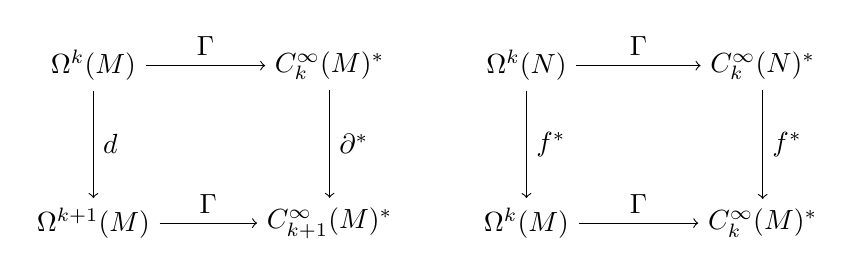
\begin{tikzpicture}
                \begin{scope}
                    \draw node (node1) at (0,0) {$\Omega^k(M)$};
                    \draw node (node2) at (3,0) {$C_k^\infty(M)^\ast$};
                    \draw node (node3) at (0,-2) {$\Omega^{k+1}(M)$};
                    \draw node (node4) at (3,-2) {$C_{k+1}^\infty(M)^\ast$};
    
                    \draw[->] (node1.east) to node[above] {$\Gamma$} (node2.west);
                    \draw[->] (node1.south) to node[right] {$d$} (node3.north);
                    \draw[->] (node2.south) to node[right] {$\partial^\ast$} (node4.north);
                    \draw[->] (node3.east) to node[above] {$\Gamma$} (node4.west);
                \end{scope}
    
                \begin{scope}[xshift=5.5cm]
                    \draw node (node1) at (0,0) {$\Omega^k(N)$};
                    \draw node (node2) at (3,0) {$C_k^\infty(N)^\ast$};
                    \draw node (node3) at (0,-2) {$\Omega^k(M)$};
                    \draw node (node4) at (3,-2) {$C_k^\infty(M)^\ast$};
    
                    \draw[->] (node1.east) to node[above] {$\Gamma$} (node2.west);
                    \draw[->] (node1.south) to node[right] {$f^\ast$} (node3.north);
                    \draw[->] (node2.south) to node[right] {$f^\ast$} (node4.north);
                    \draw[->] (node3.east) to node[above] {$\Gamma$} (node4.west);
                \end{scope}
            \end{tikzpicture}
        \end{center}
        For the left diagram we compute:
        \[
        (\Gamma \circ d)(\omega) = \left(\sigma \mapsto \int_\sigma d\omega\right) = \left(\sigma \mapsto \int_{\partial\sigma} \omega\right) = (\partial^\ast \circ \Gamma)(\omega) 
        \]
        where we used Stokes' Theorem for singular chains in the second equality. Moreover, we compute for the right diagram:
        \begin{align*}
            (\Gamma \circ f^\ast)(\omega) &= \left(\sigma \mapsto \int_\sigma f^\ast \omega\right) \\
            (f^\ast \circ \Omega)(\omega) &= \left(\sigma \mapsto \int_{f\circ\sigma} \omega\right)
        \end{align*}
        But by definition:
        \[
        \int_\sigma f^\ast \omega = \int_{\Delta^k} \sigma^\ast f^\ast \omega = \int_{\Delta^k} (f\circ\sigma)^\ast \omega = \int_{f\circ\sigma}\omega
        \]
        This completes the proof.
        \end{proof}

        \begin{lemma}
            \label{lem:natural_cochain_map2}
            The inclusion $C_k^\infty(M) \to C_k(M)$ induces a natural map of cochain complexes
            \[
                (C_k^\infty(M)^\ast,\partial^\ast) \to (C_k(M)^\ast,\partial^\ast)
            \]
        \end{lemma}
        \begin{proof}
            Obvious.
        \end{proof}

        In the lecture we have shown that the cochain maps from the above two lemmata induce isomorphisms in homology at least for open subsets of $\R^n$. A short proof of how this generalizes to all manifolds with or without boundary is given in the following theorem (which notably uses facts that we have not established in the lecture).

        \begin{theorem}
            The cochain maps from Lemma \ref{lem:natural_cochain_map1} and \ref{lem:natural_cochain_map2} induce isomorphisms in homology.
        \end{theorem}
        \begin{proof}
            
        \end{proof}